\documentclass{standalone}
\usepackage{tikz}
\usetikzlibrary{patterns,decorations.pathmorphing}
\begin{document}
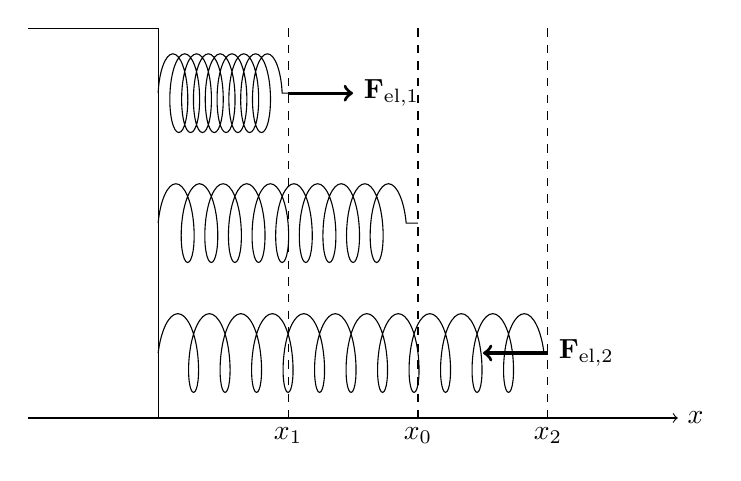
\begin{tikzpicture}[scale=1.65]
    \draw[->](-1,0)--(4,0)node[right]{$x$};
    \draw[-](0,0)--(0,3);
    \draw[-](0,3)--(-1,3);
    
    \draw[dashed](1,3)--(1,0)node[below]{$x_1$};    
    \draw[dashed](2,3)--(2,0)node[below]{$x_0$};
    \draw[dashed](3,3)--(3,0)node[below]{$x_2$};

    \draw[decoration={aspect=0.3, segment length=4mm, amplitude=5mm,coil},decorate] (0,0.5) -- (3,0.5); 
    \draw[decoration={aspect=0.3, segment length=3mm, amplitude=5mm,coil},decorate] (0,1.5) -- (2,1.5); 
    \draw[decoration={aspect=0.3, segment length=1.5mm, amplitude=5mm,coil},decorate] (0,2.5) -- (1,2.5); 

    \draw[->,very thick](1,2.5)--(1.5,2.5)node[right]{$\mathbf{F}_{\mathrm{el},1}$};
    \draw[->,very thick](3,0.5)node[right]{$\mathbf{F}_{\mathrm{el},2}$}--(2.5,0.5);
\end{tikzpicture}
\end{document}